\subsection{Architektur und Funktionsweise}
\label{sec:prototype_arch}
    Enstprechend dem Kapitel mit dem Stand der Wissenschaft wurden die Konzepte im Framework umgesetzt.
    Ausgehend von der Dokumentation des Frameworks \cite{ComposerDocs} wurde die Architektur ausgearbeitet. 
    
    Keine Standardisierung und Best Practices von Architekturen, wie in fast allen Bereichen des \gls{iot}, daher eigentlich völlig frei.
    
    \begin{figure}[H]
		\centering
		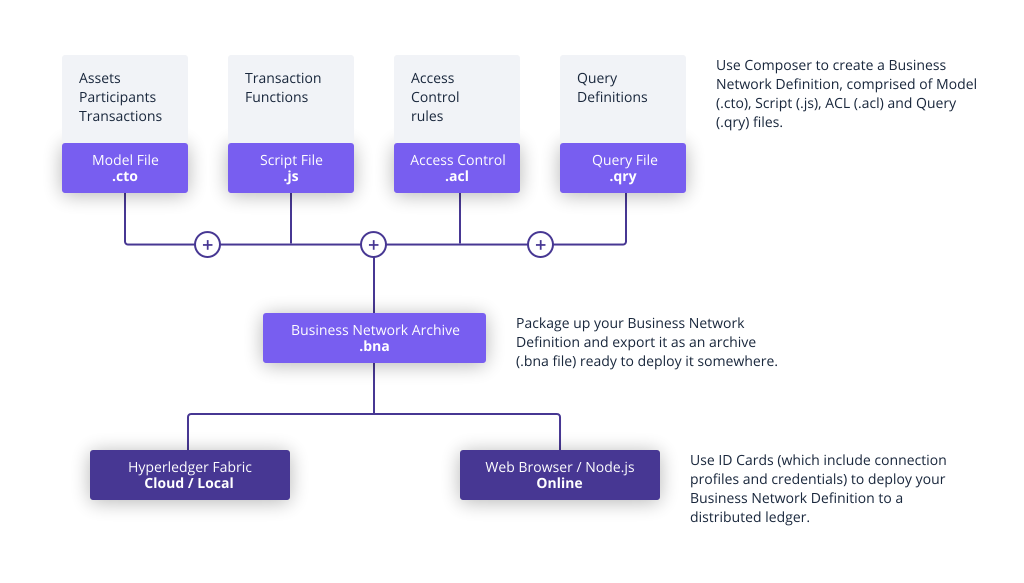
\includegraphics[width=\textwidth]{graphics/Composer-Diagram.png}
		\caption[Bestandteile einer Hyperledger Composer-Applikation]{Bestandteile einer Hyperledger Composer-Applikation\cite{ComposerDocs}}
		\label{fig:composer_arch}
	\end{figure}
    
    Notizen für den Prototypen:
    \begin{itemize}[noitemsep]
        \item Ein Asset als Token für (,,du darfst die Tür aufmachen``) je berechtigtem Nutzer \textrightarrow\ zurückverfolgbar (Accountability)
        \item Framework bietet in irgendeiner Form Access Control an?
        \item How to ensure a consistent state across all entities?...
        \item Vendor Server als Teilnehmer im Netzwerk oder nicht?
        \item Vertraulichkeit überhaupt irgendwie möglich oder durch das Konzept der Blockchain schon gar nicht?
        \item Pseudo-/Anonymisierung der Teilnehmer sinnvoll?
        \item Hyperledger biete CA für Identitäten, Authentifizierung
        \item 
    \end{itemize}
    
    \subsubsection{Konzept}
    
    \paragraph{Model File}
        Asset Types:
        \begin{itemize}[noitemsep]
            \item Door Key (kann zeitlich beschränkt sein), bei Öffnen an Schloss senden, bei Schließen wieder an Nutzer zurück \textrightarrow\ man kann sich sicher sein, dass die Tür bei 0 Token geschlossen ist.
            \item Token, der die Rolle repräsentiert?
            \item Um \gls{dos} zu vermeiden, etwas ähnliches wie Mutex-Token? z.B. wenn Tür offen ist, dann hat sie genau diesen einen Token
            \item Assets können auch zu anderen Assets oder Teilnehmern eine Beziehung haben\cite{ComposerDocs}
        \end{itemize}
        
        Participant Types:
        \begin{itemize}[noitemsep]
            \item Manufacturer
            \item Owner
            \item Guest
        \end{itemize}
        
        Transaction Types (entpricht den Funktionen, die man je nach Rolle ausführen darf):
        \begin{itemize}[noitemsep]
            \item OpenDoor
            \item User (AddUser, DeleteUser, ChangeUserRole)
            \item TimeSlot (AddTimeSlot, DeleteTimeSlot, ChangeGuestTimeSlot)
        \end{itemize}
    
    \paragraph{Transaction Functions}
    
    \paragraph{Access Control Rules}
    
    \paragraph{Query Definitions}
    
    Rollenbasiertes Zugriffskonzept
    \begin{itemize}[noitemsep]
        \item 
    \end{itemize}